%\documentclass[a4paper,10pt]{report}
\documentclass[11pt,titelpage]{scrartcl}
\usepackage[utf8]{inputenc}
\usepackage[ngerman]{babel}
\usepackage{graphicx}
\usepackage{fancyhdr}
\usepackage{fancyref}
\usepackage{lscape}
\usepackage{listings}

%must be before gloassary stuff\usepackage{hyperref}
\usepackage[toc]{glossaries}

%\makeglossaries
%
\newglossaryentry{Buildystem}
{
  name=Buildystem,
  description={Linux Mint 17, Java JDK 1.8.1, Intellij 2016.3.5, JavaFx Scene Builder 2.0}
} 

\newglossaryentry{Referenzsystem}
{
  name=Referenzsystem,
  description={Linux Mint 17, Java JRE 1.8.1, Derby10.13.1.1}
} 

\newglossaryentry{Programmstart}
{
  name=Programmstart,
  description={Prozess welcher das Programm initialisiert}
} 


 
\newglossaryentry{Standarddatenbank}
{
  name=Standarddatenbank,
  description={Derby, MySQL, SQLite}
} 


\newglossaryentry{JPA Driver}
{
  name=JPA Driver,
  description={JPA Driver und JPA Module sind Opensource CMS (Content Management Systeme)}
} 

\newglossaryentry{Benutzer}
{
  name=Benutzer,
  description={Ein Benutzer ist ein Mensch, welcher unser Programm benutzt. Falls nicht anders erwähnt, muss dieser
  weder registriert noch angemeldet sein}
} 


\newglossaryentry{Event}
{
  name=Event,
  description={Ein Event ist ein Ereignis, welches zu einem bestimmten Zeitpunkt stattfindet}
} 

\newglossaryentry{Einzelevent}
{
  name=Einzelevent,
  description={Ein Einzelevent ist ein Event, welches nicht periodisch wiederkehrend stattfindet, also können auch
   ein Treffen, welches unregelmässig stattfindet zu einem Einzelevent werden.}
} 

\newglossaryentry{GUI}
{
  name=GUI,
  description={Graphical User Interface. Ein GUI ist eine Graphische Benutzeroberfläche. Sie hat die Aufgabe das
  Programm für den Benutzer bedienbar zu machen}
} 

\newglossaryentry{CLI Wikipedia}
{
  name=CLI,
  description={Command Line Interface. Das CLI ist die Konsole, wird oft auch Terminal gennant. Sie steuert eine
  Software mittels Textmodus. Je nach Betriebssystem wird die Kommandozeile von einer Shell ausgewertet und die
  entsprechende Funktion ausgeführt.
  - Wikipedia}
}

\newglossaryentry{Shell}
{
  name=Shell,
  description={In der Informatik bezeichnet man als Shell die Software, die den Benutzer mit dem Computer verbindet.
  Die Shell ermöglicht zum Beispiel, Kerneldienste zu nutzen und sich über Systemkomponenten zu informieren oder sie zu
  bedienen. Die Shell ist in der Regel ein Teil des Betriebssystems.
  - Wikipedia
  }
}


\newglossaryentry{API}
{
  name=API,
  description={Application Programming Interface. Ein API ist ein Programmteil, der von einem Softwaresystem anderen
  Programmen zur Anbindung an das System zur Verfügung gestellt wird
  - Wikipedia}
} 

\newglossaryentry{Notification}
{
  name=Notification,
  description={Eine Notification ist eine Aktion des Programms, die den Benutzer auf ein Event aufmerksam machen soll.}
} 

\newglossaryentry{Konfiguration}
{
  name=Konfiguration,
  description={Die Konfiguration kann ein Programm auf die Bedürfnisse des Nutzers anpassen. So kann man beispielsweise
   die Spracheinstellung konfigurieren.}
} 

\newglossaryentry{Filtern}
{
  name=Filtern,
  description={Filtern bedeutet, dass man gewisse Informationen nur darstellt, wenn diese eine oder mehrere bestimmte Charakteristiken aufweist. So ist es zum Beispiel möglich Events nach Kategorein zu filtern, so dass man nur Events aus einer bestimmten Kategorie sehen kann.}
} 


\newglossaryentry{Kategorien}
{
  name=Kategorien,
  description={Eine Kategorie hilft die Events zu klassieren. Denkbare Kategoreien sind zum Beispiel: Arbeit, Freizeit, Persönlich,Familie,Wichtig,Sportverein... }
} 

\newglossaryentry{Android}
{
  name=Android,
  description={Android ist ein Betriebssystem für Mobile Geräte wie Smartphones, Tablets etc.
   Es wird von der von Google gegründeten Open Handset Alliance entwickelt}
}

\newglossaryentry{Notification Infrastruktur}
{
  name=Notification Infrastruktur,
  description={Einige Desktop Environments  wie Gnome oder KDE bieten eine eigene Notification Infrastruktur, diese erlaubt es ``Pop-Ups'' durch Systemkomponenten darzustellen. KDE benutzt dies beispielsweise um auf einen Niedrigen Batterieladezustand hinzuweisen. Auch andere Programme können diese Notification Infrastruktur nutzen. }
} 

\newglossaryentry{Desktop Environment}
{
  name=Desktop Environment,
  description={Deskto Environment, ist eine Graphsche Benutzeroberfläche für das Betriebssystem. Vorallem unter
  Unixoiden Betriebssystemen, hat man eine grosse Auswahl an Desktop Environments (KDE, gnome, w3..)}
} 

\newglossaryentry{Cronjob}
{
  name=Cronjob,
  description={Cronjob ist ein Unix Dienst, welcher dazu dient zu einem bestimmten Zeitpnkt Ereignisse auszulösen.}
} 



\newglossaryentry{IFTTT}
{
  name=IFTTT,
  description={IFTTT (die Abkürzung von If This Then That, ausgesprochen „ift“ wie in „Gift“[1]) ist ein Dienstanbieter,
  der es Benutzern erlaubt, verschiedene Webanwendungen (zum Beispiel Facebook, Evernote, Dropbox usw.) mit einfachen
  bedingten Anweisungen zu verknüpfen.
   -Wikipedia}
} 








% Title Page
\title{Alarm Clock }
\author{Jonathan Hyams \\Pascal Schmalz}
%\titlehead{\centering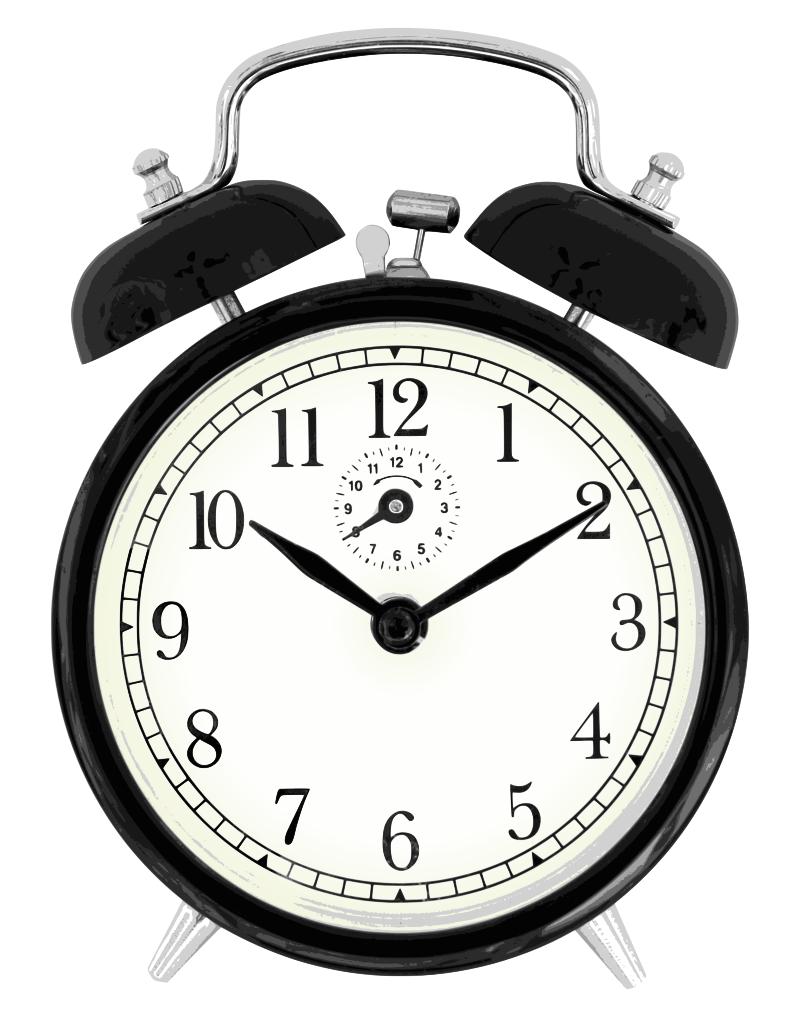
\includegraphics[width=6cm]{img/clock.png}}

%Make the Header
\makeatletter
\let\runauthor\@author
\let\runtitle\@title
\makeatother
\rhead{\runauthor}
\chead{\runtitle}
%\lhead{\begin{picture}(0,0) \put(0,0){
\includegraphics[scale=0.5]{img/bfh.png}} \end{picture}}



\begin{document}

\thispagestyle{empty}
\maketitle
\pagebreak
\tableofcontents

\pagestyle{fancy}


\begin{abstract}
\end{abstract}
\pagebreak

\section{Zweck des Dokument}
\section{Architektur}
Unser Programm implementiert ein MVC Pattern. Die Komponenten Model und Controller sind als Java Pakete schnell ersichtlich. Die View wird aber nicht in einem Java-Packet ausprogrmamiert. Da wir JavaFx nutzen, wird die View durch JavaFx definiert. Die Implementierungsdetails findet man unter resources/mainWindow.fxml. Auch das Notification Paket könnte man zur View zählen.

Die wichtigsten Komponenten sieht man in der Abbildung Systemübersicht.
\begin{landscape}
\begin{figure}
  \centering
    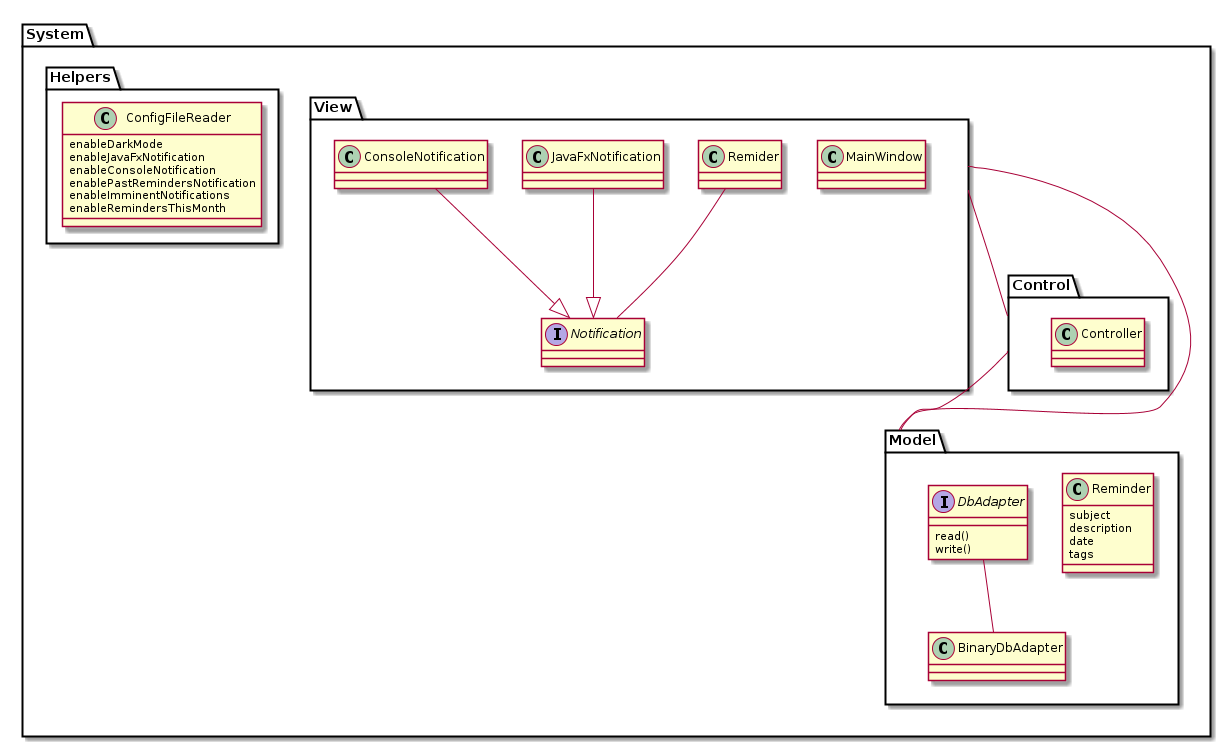
\includegraphics[width=1\textwidth]{../uml/uebersicht01.png}
  \caption{Systemübersicht}
  \label{fig:overview}
\end{figure}
\end{landscape}

Spezielle Aufmerksamkeit bedarf das Auslösen eines Reminders.
\subsection{Auslösen Notification}

Der Poller stösst regelmässig den NotificationHandler an.
In diesem werden Kriterien definiert, nach welchen die Reminders gefiltert werden, zum Beispiel alle Reminders, welche in der nächsten Stunde beginnen.



Dann wird über alle Reminders iteriert. Jedem Reminder, wird dabei der Filter an die NotifyIf() Funktion übergeben.
Der Reminder testet nun anhand des Filters selbstständig, ob das Kriterium zutrifft oder nicht. Dazu nutzt er seine meetsCriteria() Funktion.
Falls diese eine positive Antwort gibt, wird die doNotify() Funktion aufgerufen. Diese lädt eine Liste mit den Notifications, welche im ConfigReader definiert wird.
Jeder dieser Notifications wird dem Reminder übergeben, welcher die Notifications auslösen will. Dann wird die Notifications abgesendet.

\subsection{Konfiguration}
Die Konfigurationsmöglichkeiten sind im ConfigReader File zentral gelöst. Somit wird es später auch leicht möglich, über diese Klasse ein Konfigurationsfile
einzulesen, und die entsprechenden Komponenten zu konfigurieren.

\section{Controller}
\subsection{Class: Controller}
Die Controller Klasse arbeitet eng mit der mainWindow.fxml Datei zusammen. Würde man dieser Klasse den Namen ändern, so müsste man im fxml das Statement
\begin{lstlisting}
fx:controller="alarmClock.controller.Controller"
\end{lstlisting}
anpassen.

In der FXML Datei hat jedes Item im GUI eine ID. Damit man im Java Code auf die jeweiligen Komponenten zugreifen kann, hängt man bei der Initialisierung ein @FXML tag dran,
damit das Programm weiss, mit welchen Komponenten er umgeht.
\begin{lstlisting}
    @FXML
    private TextField subjectField;
\end{lstlisting}

\begin{lstlisting}
  <TextField fx:id="subjectField" prefHeight="25.0" prefWidth="107.0" promptText="Subject"\"></TextField>
\end{lstlisting}

Da in beiden Dateien subjectField gleich heisst, kann man nun problemlos im Java Code auf das gewünschte Feld zugreifen.
Man kann auch definieren, welche Methode aufgerufen werden soll, wenn man bsp. einen Button drückt. Für addButtonPressed() und rmButtonPressed() haben wir das so gemacht.

\begin{lstlisting}
onAction="#addButtonPressed"
\end{lstlisting}

Im tag des AddButtons (in der fxml Datei) nennen wir die Methode die aufgerufen werden soll "addButtonPressed". Damit der Java-Compiler merkt, dass er eine FXML Kompenente
suchen muss, fügen wir vor der Methode noch ein @FXML tag hinzu.
\begin{lstlisting}
    @FXML
        public void addButtonPressed() {
        ...
        }
\end{lstlisting}

Die addButtonPressed() Methode fügt Reminders in die Tabelle hinzu, solange der Input legal ist. Das heisst die Felder dürfen nicht leer sein (getValue != null).
Wenn der Button gedrückt wird, werden die Felder wieder leer gemacht.


Die rmButtonPressed() Methode löscht Reminders, die man mit der Maus selektiert hat.

\begin{lstlisting}
    ReminderList reminderSelected;
    reminderSelected = new ReminderList(reminderTable.getSelectionModel().getSelectedItems());
    model.removeReminders(reminderSelected);
\end{lstlisting}

Wir kreieren eine Liste und fügen alle selektierten Reminders hinzu, und löschen diese dann aus der Tabelle.


Die Methode Initialize haben wir reingenommen, da JavaFX Komponenten erst nach dem Ausführen des Konstruktors erstellt werden. Sie dient als Konstruktor.
\begin{lstlisting}
  BooleanBinding addBinding = subjectField.textProperty().isNotEmpty().and(datePickerField.valueProperty().isNotNull());
  addButton.disableProperty().bind(addBinding.not());
\end{lstlisting}
Das Binding oben deaktiviert den addButton wenn der Input nicht valid ist.

\begin{lstlisting}
reminderTable.getSelectionModel().setSelectionMode(
                SelectionMode.MULTIPLE
        );
\end{lstlisting}
Dies erlaubt dem User mehrere Items in der Tabelle zu markieren.

Um die Initialisierung des Models mussten wir noch einen try/ catch Block hinzufügen, da das Model Exceptions werfen kann.

\begin{lstlisting}
reminderTable.setItems(model.getReminders());
\end{lstlisting}
setItems() fügt beim Starten des Programms Reminders in die Tabelle, die in der DB gespeichert wurden.

\subsection{Class: DateTimePicker}
Die DateTimePicker Klasse haben nicht wir geschrieben. Wir haben diese Klasse auf StackOverflow gefunden. Da JavaFX nur einen DatePicker zur Verfügung stellt, mussten wir
diesen benutzen. Es handelt mit LocalDateTime Objekten, die auch die Uhrzeit mitgeben.
Der DateTimePicker gibt zwei sehr praktische Felder zur Verfügung: Das dateTimeValue, welches das Datum inklusiver Zeit enthält, und das valueProperty, welches nur das Datum enthält.
Im Konstruktor wird ein Listener erstellt, welcher das dateTimeValue überschreibt, wenn der User im GUI etwas ändert.
In der DateTimePicker Klasse wurde noch eine zweite Klasse hinzugefügt, der InternalConverter. Dieser holt den String aus dem DateTimePicker und parsed es zu einem LocalDateTime
Objekt.

\section{Filtering}
\subsection{ Higher Order Functions}
  Die Marketingabteilung von Oracle behauptet gerne Java seie auch Funktional. Higer Order Functions werden aber nicht wirklich unterstützt. 
  TODO wikipedia Higer Order function. 
  Funktionen als Return Values oo
  
  Java unterstüzt leider keine Higher order functions. Man kann also keine Funktion als Inputparameter übergeben.
  Mittels Lambdas ist es lediglich möglich, die eine Funktion ausführen zu lassen und den Rückgabewert als Inputparameter weiter zu verwenden. Dies erlaubt eine kompaktere Notation. Dies reicht uns aber nicht, da wir den Remindern eine Funktion übergeben möchten, mit welcher jeder Reminder selber testet ob er eine Notification absenden soll. 
  
  \subsection{echte Higher Order Functions in Java}
  Um dies zu erreichen haben wir eine Form von Higher Order Functions mit Objekten nachgebaut. 
  Ein CriteraTester ist ein Objekt, welches als Wrapper für eine Funtion dient. Anstelle dieser Funktion übergibt man nun diesen FunktionsWrapper als Inputparameter. Somit konnten wir Funktionen als Inputparameter mittels Objektorientierten prinzipien nachbauen.
  Man muss nun für jede Funktion ein Objekt erstellen, welches das Interface CriteraTester implementiert.Und die Filterfunktion isTrue implementieren.
  Funktionen als Rückgabewert kann man so aber noch nicht wirklich nachbauen. Für uns war das aber nicht nötig.
  
  Dank den oben erwähnten Lambdas kann man dies auch elegan on the Fly erledigen. Da es aber vorkommen kann dass man einen Filter mehrmals benutzt, habe wir uns entschieden die Filter jeweils als eigene Klassen zu implementieren.
  \subsection{Code Beispiel}
  
       \begin{lstlisting}
       Reminder r;
       Collection<CriteriaTester> criteria = new ArrayList<>();
        criteria.add(new IsPassed());
         //     example how CriteraTester can be written on the fly
        //pus this to documentation
        criteria.add(
                r -> (!r.getTags().contains("hidden"))
        );
        //This lets the Reminder send a notification if the Reminder meets the criterias 
        //The first criteia it must pass it th IsPassed()
        //the second criteria is defined on the fly on  line number TODO x. it tests if it contains the tag "hidden"
        
     
        r.notifyIf(criteria);

       \end{lstlisting}
\section{Notification}
\subsection{Interface: Notification}
Das NotificationInterface gibt zwei Methoden vor:

\begin{lstlisting}
   void setReminder(Reminder reminder);
\end{lstlisting}
setReminder übergibt den Reminder, für den man eine Notifcation erstellen will.

\begin{lstlisting}
   void send();
\end{lstlisting}
send() wird vom Reminder aufgerufen, und zeigt dem User die Notification. Es gibt verschiene Arten von Notifications.
JavaFxNotification ist das Popup das den Reminder aufzeigt, der gerade aktuell ist. MultireminderNotification
zeigt alle schon vergangenen Reminders, und ConsoleReminder zeigt auf der Konsole (Shell) einen Reminder.
All diese Notification-Klassen implemenetieren Notification.


\subsection{Class: ConsoleNotification}
ConsoleNotification hat einen leeren Konstruktor aus mehreren Gründen. Wir haben ihn ähnlich wie den JavaFxNotification aufebaut,
und JavaFX verlangt einen leeren Konstuktor, also haben wir ihn hier beibehalten. Auch haben wir einen Konstruktor mit einem Reminder im Parameter gemacht,
also war der DefaultKonstruktor überschrieben.
Der ConfigReader benutzt diese Klasse auch (inklusive dem leeren Konstruktor) und benötigt keinen direkten Reminder, also haben wir ihn so stehen lassen.

Der Konstruktor mit dem Reminder im Parameter und die setReminderMethode machen eingentlich genau das gleiche. setReminders wird noch vom Notication Interface verlangt.
Die send() Methode wird vom Reminder aufgerufen wenn die Zeit soweit ist. Sie druckt einfach die toString() Methode des Reminders auf die Konsole.


\subsection{Class: JavaFxNotification}
Die JavaFxNotification Klasse ist identisch mit der ConsoleNotification, nur die send() Methode ist anders.
Die send() Methode enthält die statische Methode:
\begin{lstlisting}
  Platform.runLater( () -> {...});
\end{lstlisting}
In den geschweiften Klammern wird ein Popup Fenster erstellt. Da wir mit Threads arbeiten, und diese Popups verspätet aufgerufen werden,
müssen wir das GUI in das Platform.runlater einpacken. Die JavaDoc vom runlater() sagt 'Run the specified Runnable on the JavaFX Application
Thread at some unspecified time in the future [...]',
und das ist genau was wir brauchen. Lässt man es weg, bekommt man dutzende von Exceptions.

\begin{lstlisting}
  {
Stage stage = new Stage();
                    label = new Label("Hello: " + reminder.toString());
                    Button okButton = new Button("Ok");
                    okButton.setOnAction(e -> {
                        stage.close();
                    });
                    VBox pane = new VBox(10, label, okButton);
                    pane.setAlignment(Pos.CENTER);
                    pane.setPadding(new Insets(10));
                    Scene scene = new Scene(pane);
                    stage.setTitle("Reminder");
                    stage.setScene(scene);
                    stage.setResizable(false);
                    stage.show();
    }
\end{lstlisting}
Der Code in den geschweiften Klammern macht ein simples JavaFX Fenster das den Reminder aufzeigt. Das Label wird mit der reminder.toString() Methode überschrieben. Dem okButton schliesst das Fenster wenn man ihn drückt. Die Komponenten Button und Label tun wir in ein VBox Behälter und machen ihn noch ein bisschen schöner mit setAlignment() und setPadding().


\subsection{Class: MultiReminderNotification}
MultiReminderNotification zeigt alle schon vergangenen Reminder in einem einzigen Fenster an. Der Aufbau der Klasse ist genau gleich wie in JavaFxNotification und ConsoleNotification, nur dass anstatt einem Reminder hat er eine Liste von Reminder.
\begin{lstlisting}
private Collection<Reminder> reminders;

String remindersText = "";
                    int i = 0;
                    for (Reminder r : reminders) {
                        remindersText += "Passed Event No " + ++i + ":\n";
                        remindersText += r.toString() + "\n";
                        System.out.print("added" + r.toString());
                    }
\end{lstlisting}
Hier Iterieren wir durch alle Reminders in der Tabelle und fügen sie zum Label hinzu. Die Reminders sind in der reminders Liste. Damit wir nicht alle Reminders in diesem Popup habem, sonder nur die die bereits vergangen sind oder schon sehr bald erscheinen, werden diese im NotificationHandler noch gefiltert.
Die Methoden dazu wären folgende:
\begin{lstlisting}
criteria.add(new IsPassed());
criteria.add(new IsThisYear());
\end{lstlisting}

\subsection{Class: NotificationHandler}
TODO

\section{Resources}
\subsection{Resources}
Die Resourcen die wir gebraucht haben waren:
\begin{itemize}
  \item Java
  \item JavaFX
  \item IntelliJ
  \item Atom
  \item Latex
  \item TornadoFX-Controls Plugin
  \item Git
  \item Github
  \item JUnit

\end{itemize}

\section{Tests}
\subsection{Tests}
Unseren Code haben wir Mittels JUnit getestet. Für das GUI hätte man mit einem Testing Framework arbeiten können, aber davor wurde uns im
Kurs Software Engineering and Design abgeraten.

\section{Tools}
Um die  Versionierung der Dokumentation automatisch generieren zu lassen, haben wir LaTeX so mit Scripts erweitert, so dass die git Head Versionsnummer
direkt ins Dokument eingefügt wird. Somit bleibt diese Information auch auf einem Ausdruck akkurat.

\section{Main}
 
Dies ist die Klasse die die Main methode enthält. Sie erbt von der Klasse Application, da Sie das JavaFX-GUI launched.
\begin{lstlisting}
   Parent root = FXMLLoader.load(getClass().getResource(windowName));
\end{lstlisting}
windowName ist der Name der fxml Datei (mainWindow.fxml), in der das Aussehen und der Controller definiert wird. "mainWindow.fxml" befindet sich im package "resources".


\section{Versionskontrolle}
Manuelle Version: 1.0.0
\\

\noindent
Automatische Versionierung:
%\immediate\write18{../script/versionInfo.sh}
%Fetching version information failed. Please enable shell-escape in your \LaTeX \~  compiler.

%\immediate\write18{../script/cleanup.sh}
%\immediate\write18{../script/clean.sh}







\end{document}
